
% ===================================================================
% FILE: Lezione18.tex
% ===================================================================

% --- Definizioni Locali (Compatibilità) ---
% (Rimosso codebox locale poiché definito in main.tex)

\part{Lezione 18: Strutture Dati Lineari}

\section{Liste (Linked Lists)}

Le liste rappresentano una struttura dati fondamentale per la gestione di collezioni dinamiche di elementi.

\begin{concept}{Definizione e Struttura}
Una lista è una sequenza di nodi dove ogni elemento è \textbf{virtualmente concatenato} ma non necessariamente contiguo in memoria. Non è necessario conoscere la dimensione a priori (numero di elementi necessari).

La struttura di base di un nodo comprende:
\begin{itemize}
    \item Un campo dati (informazione).
    \item Un campo \texttt{NEXT} che punta all'elemento successivo.
\end{itemize}
La lista è accessibile tramite un puntatore alla testa (\texttt{HEAD}).
\end{concept}

\subsection{Tipologie e Vantaggi}
\begin{itemize}
    \item \textbf{Liste Semplici:} Collegamento unidirezionale (\texttt{NEXT}).
    \item \textbf{Liste Doppie:} Ogni nodo possiede due puntatori: uno al successivo (\texttt{NEXT}) e uno al precedente (\texttt{PREC}).
\end{itemize}

\textbf{Vantaggi rispetto agli Array:}
Le liste sono molto comode per effettuare inserimenti ed eliminazioni in posizioni intermedie, operazioni che in un array risulterebbero scomode (richiedendo lo shift degli elementi).

\begin{center}
\begin{tikzpicture}[list/.style={rectangle split, rectangle split parts=2,
    draw, rectangle split horizontal}, >=stealth, start chain]

  \node[list, on chain] (A) {Dati \nodepart{second} Next};
  \node[list, on chain] (B) {Dati \nodepart{second} Next};
  \node[list, on chain] (C) {Dati \nodepart{second} $\emptyset$};

  \draw[->] let \p1 = (A.two), \p2 = (A.center) in (\x1,\y2) -- (B);
  \draw[->] let \p1 = (B.two), \p2 = (B.center) in (\x1,\y2) -- (C);
  
  \node[left=of A, anchor=east] {HEAD};
  \draw[->] ($(A.west)+(-0.5,0)$) -- (A.west);
\end{tikzpicture}
\end{center}

---

\section{Pile (Stack)}

La Pila è un insieme dinamico gestito con politica \textbf{LIFO (Last In First Out)}: si entra e si esce solo dalla "cima".

\begin{concept}{Operazioni Fondamentali}
Una pila supporta le seguenti operazioni, tutte con complessità $\Theta(1)$:
\begin{itemize}
    \item \textbf{PUSH:} Aggiunge un elemento in cima alla pila.
    \item \textbf{POP:} Rimuove l'elemento in cima alla pila.
    \item \textbf{QUERY:}
    \begin{itemize}
        \item \texttt{ISEMPTY}: Verifica se la pila è vuota.
        \item \texttt{TOP}: Restituisce il valore dell'elemento in cima senza rimuoverlo.
    \end{itemize}
\end{itemize}
\end{concept}

\subsection{Implementazione con Array}
Struttura: $\text{PILA} = \langle A, \text{TOP} \rangle$.
\begin{itemize}
    \item \texttt{TOP}: indice che varia tra $0$ e $n-1$. Vale $-1$ se la pila è vuota.
    \item \textbf{Svantaggio:} Bisogna definire a priori la dimensione massima ($A.length$).
\end{itemize}

\begin{codebox}{Algoritmi Pila (Array)}
\textbf{ISEMPTY(PILA)}
\begin{verbatim}
IF (TOP < 0) THEN RETURN TRUE
ELSE RETURN FALSE
\end{verbatim}

\textbf{TOP(PILA)}
\begin{verbatim}
IF ISEMPTY(PILA) THEN error
ELSE RETURN A[TOP]
\end{verbatim}

\textbf{PUSH(PILA, X)}
\begin{verbatim}
TOP = TOP + 1
IF (TOP >= A.length) THEN error (Overflow)
A[TOP] = X
\end{verbatim}

\textbf{POP(PILA)}
\begin{verbatim}
IF ISEMPTY(PILA) THEN error (Underflow)
ELSE
    X = A[TOP]
    TOP = TOP - 1
    RETURN X
\end{verbatim}
\end{codebox}

\begin{explanation}{Dettagli Implementativi (Stack Array)}
\begin{enumerate}
    \item \textbf{TOP}: Mantiene l'indice dell'ultimo elemento inserito.
    \item \textbf{PUSH}: Incrementa prima \texttt{TOP}, poi scrive. Se \texttt{TOP} supera la capacità, si ha \textit{Overflow}.
    \item \textbf{POP}: Legge l'elemento a \texttt{TOP} e poi decrementa. Se \texttt{TOP} diventa negativo, lo stack è vuoto (Underflow).
\end{enumerate}
\end{explanation}

\begin{center}
\begin{tikzpicture}[scale=0.8]
    \node[draw, minimum width=2cm, minimum height=0.6cm] (c1) at (0,0) {Data A};
    \node[draw, minimum width=2cm, minimum height=0.6cm, above=0cm of c1] (c2) {Data B};
    \node[draw, minimum width=2cm, minimum height=0.6cm, above=0cm of c2] (c3) {};
    \node[right=0.5cm of c2] {$\leftarrow$ TOP};
    \node[above=0.5cm of c3] {Stack (Array)};
\end{tikzpicture}
\end{center}

\subsection{Implementazione con Lista}
Struttura gestita tramite un puntatore \texttt{TOPER} che indica la testa della lista (cima della pila). Non ha limiti di dimensione fissa.

\begin{codebox}{Algoritmi Pila (Lista)}
\textbf{ISEMPTY(TOPER)}
\begin{verbatim}
IF (TOPER == NULL) THEN RETURN TRUE
ELSE RETURN FALSE
\end{verbatim}

\textbf{PUSH(TOPER, X)} (X è il nuovo nodo)
\begin{verbatim}
X.next = TOPER
TOPER = X
\end{verbatim}

\textbf{POP(TOPER)}
\begin{verbatim}
IF ISEMPTY(TOPER) THEN error
val = TOPER.key
TOPER = TOPER.next
RETURN val
\end{verbatim}
\end{codebox}

\begin{explanation}{Dettagli Implementativi (Stack Lista)}
\begin{itemize}
    \item Non esiste limite di dimensione (se non la memoria).
    \item \textbf{PUSH}: Inserimento in testa ($O(1)$). Il nuovo nodo punta alla vecchia testa.
    \item \textbf{POP}: Rimozione in testa ($O(1)$). Si aggiorna \texttt{TOPER} al successivo.
\end{itemize}
\end{explanation}

---

\section{Code (Queue)}

La Coda è un insieme dinamico gestito con politica \textbf{FIFO (First In First Out)}: si entra solo dalla coda (\texttt{tail}) e si esce solo dalla testa (\texttt{head}).

\subsection{Implementazione con Array Circolare}
Struttura: $\text{CODA} = \langle A, \text{head}, \text{tail} \rangle$.
L'array è trattato come circolare usando l'aritmetica modulare.

\begin{concept}{Gestione Indici Circolari}
Gli indici avanzano modulo la lunghezza dell'array ($A.length$).
Esempio calcolo indici:
$$ (6+1) \pmod{7} = 0 $$
$$ (3+1) \pmod{7} = 4 $$
\end{concept}

\begin{codebox}{Algoritmi Coda (Array Circolare) - $\Theta(1)$}
\textbf{ISEMPTY(CODA)}
\begin{verbatim}
RETURN (head == tail)
\end{verbatim}

\textbf{FIRST(CODA)}
\begin{verbatim}
IF ISEMPTY(CODA) THEN error
ELSE RETURN A[head]
\end{verbatim}

\textbf{ENQUEUE(CODA, X)}
\begin{verbatim}
// Controllo Overflow (Coda piena se tail+1 tocca head)
IF (head == (tail + 1) % A.length) THEN error
A[tail] = X
tail = (tail + 1) % A.length
\end{verbatim}

\textbf{DEQUEUE(CODA)}
\begin{verbatim}
IF ISEMPTY(CODA) THEN error
ELSE
    X = A[head]
    head = (head + 1) % A.length
    RETURN X
\end{verbatim}
\end{codebox}

\begin{explanation}{Logica Coda Circolare}
L'uso del \textbf{modulo} (\texttt{\%}) permette di riutilizzare gli spazi liberi all'inizio dell'array quando la coda avanza.
\begin{itemize}
    \item \texttt{tail}: Punta alla prima cella \textit{libera}.
    \item \texttt{head}: Punta al primo elemento valido.
    \item \textbf{Coda Piena}: Se avanzando \texttt{tail} si raggiunge \texttt{head} ($tail+1 == head$).
\end{itemize}
\end{explanation}

\begin{center}
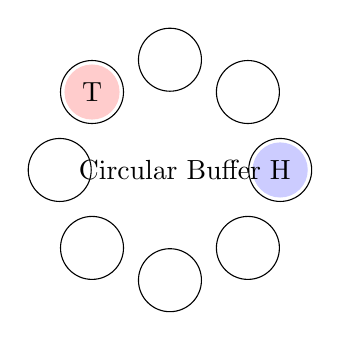
\begin{tikzpicture}[scale=0.7]
    \foreach \x in {0,1,...,7}
       \node[draw, circle, minimum size=0.8cm] (n\x) at (\x*45:2cm) {};
    \node[fill=blue!20, circle, minimum size=0.7cm] at (0:2cm) {H};
    \node[fill=red!20, circle, minimum size=0.7cm] at (135:2cm) {T};
    \node at (0,0) {Circular Buffer};
\end{tikzpicture}
\end{center}

\subsection{Implementazione con Lista}
Manteniamo due puntatori: \texttt{head} (per estrazione) e \texttt{tail} (per inserimento).

\begin{codebox}{Algoritmi Coda (Lista)}
\textbf{ISEMPTY(head, tail)}
\begin{verbatim}
IF (head == NULL) THEN RETURN TRUE
ELSE RETURN FALSE
\end{verbatim}

\textbf{ENQUEUE(head, tail, X)}
\begin{verbatim}
IF ISEMPTY(head, tail) THEN
    head = X
ELSE
    tail.next = X
tail = X  // Aggiornamento della coda (implicito ma necessario)
\end{verbatim}

\textbf{DEQUEUE(head, tail)}
\begin{verbatim}
IF ISEMPTY(head, tail) THEN error
ELSE
    val = head.key
    IF (head == tail) THEN tail = NULL // Caso svuotamento coda
    head = head.next
    RETURN val
\end{verbatim}
\end{codebox}

\begin{explanation}{Gestione coda con Lista}
Manteniamo due puntatori per garantire operazioni $O(1)$:
\begin{itemize}
    \item \textbf{ENQUEUE}: Inserisce in coda (\texttt{tail}). Aggiorna \texttt{tail.next} e poi \texttt{tail}.
    \item \textbf{DEQUEUE}: Rimuove dalla testa (\texttt{head}). Se la lista si svuota, bisogna aggiornare anche \texttt{tail} a NULL.
\end{itemize}
\end{explanation}



